\documentclass{beamer}
\usepackage{natbib}
\usepackage{hyperref}
\usepackage[utf8]{inputenc}
\usetheme{Madrid}
\usepackage{amsthm}
\usepackage{amsmath}
\usepackage{amsfonts}
\usepackage{subcaption}


\newcommand{\len}{\text{len}}
\newcommand{\amin}{\text{argmin}}
\newcommand{\aslv}{\arg\text{solve}}
\newcommand{\diag}[1]{\text{diag}\{#1\}}
\newcommand{\trace}[1]{\text{tr}\left\{#1\right\}}
\newcommand{\expect}[1]{\mathbb{E}[#1]}
\newcommand{\expectb}[1]{\mathbb{E}\left[#1\right]}
\newcommand{\expectw}[2]{\mathbb{E}_{#2}\left[#1\right]}
\newcommand{\prob}[1]{\mathbb{P}(#1)}
\newcommand{\probb}[1]{\mathbb{P}\left(#1\right)}
\newcommand{\var}[1]{\text{Var}(#1)}
\newcommand{\varb}[1]{\text{Var}\left(#1\right)}
\newcommand{\se}[1]{\text{se}(#1)}
\newcommand{\reals}{\mathbb{R}}
% interval
\newcommand{\ii}[1]{A_{#1}}     
% \newcommand{\abs}[1]{\left\lvert#1\right\rvert}
\newcommand{\func}[2]{#1{(#2)}}
\newcommand{\abs}[1]{\lvert#1\rvert}
\newcommand{\absb}[1]{\left\lvert#1\right\rvert}
\newcommand{\rank}[1]{\text{rank}(#1)}
\newcommand{\norm}[1]{\lVert#1\rVert}
\newcommand{\normb}[1]{\left\lVert#1\right\rVert}
\newcommand{\LNorm}[1]{{\lVert#1\rVert}}
\newcommand{\LTwonorm}[1]{{\lVert#1\rVert}_2}
\newcommand{\LTwonormb}[1]{{\left\lVert#1\right\rVert}_2}
\newcommand{\lone}{\ell_1}
\newcommand{\ltwo}{\ell_2}
\newcommand{\innerprod}[2]{\left\langle#1,#2\right\rangle}
\renewcommand{\dim}[1]{\text{dim}{\left(#1\right)}}
\newcommand{\doubleline}[2]{\begin{tabular}{@{}l@{}} #1 \\ #2\end{tabular}}
\newcommand{\tripleline}[3]{\begin{tabular}{@{}l@{}} #1 \\ #2\\ #3\end{tabular}}
\newcommand{\quadline}[4]{\begin{tabular}{@{}l@{}} #1 \\ #2\\ #3\\ #4\end{tabular}}
\newcommand{\abbrv}[2]{#1 (#2)}
\newcommand{\pckg}[1]{\texttt{#1}}

% Notation
\newcommand{\trst}{R}
\newcommand{\trcard}{r}
\newcommand{\trcoef}{{\beta^*}}
\newcommand{\Lassoest}{\hat{\beta}(\lambda)}
\newcommand{\Lassoestarg}[1]{\hat{\beta}(#1)}
\newcommand{\modelset}{\mathcal{M}}
\newcommand{\inprob}{\overset{p}{\to}}
\newcommand{\indist}{\overset{d}{\to}}


%Information to be included in the title page:
\title[``Plus/minus'' CIs]{``Plus/minus'' confidence intervals and thresholding}
\author[]{P. Zietkiewicz}
\date{\today}



\begin{document}

\frame{\titlepage}

\begin{frame}
	\frametitle{Table of contents}
	\tableofcontents
\end{frame}

\begin{frame}
  \frametitle{Summary of~\citet{chee:2023}}
  \begin{itemize}
  \item $(Y, X) \in \reals^d \times \reals^p$ and $D_N = \{(Y_i, X_i): i=1,\dots,N\}$
    \begin{align*}
      \theta_* &= \amin_{\theta \in \Theta} \expect{\ell(\theta, Y, X)}\\
      \hat{\theta}_N &= \amin_{\theta \in \Theta} \sum_{i=1}^N\ell(\theta, Y_i, X_i)\\
      F_* &= \expect{\nabla \ell(\theta, Y, X) \nabla \ell(\theta, Y, X)^\top}\\
    \end{align*}
  \item SGD: $\theta_n = \theta_{n-1} - \gamma_n \nabla \ell(\theta_{n-1}; Y_{i}, X_{i})$ for $i=1,\dots,N$ and $\gamma_n$ is the learning rate typically $\gamma_n = \gamma_1 / n$. Let $\theta_N$ be the one-pass estimator of $\theta_*$.
  \item Advantages of one-pass over multi-pass: (1) Asymptotic covariance matrix is known in closed form (2) Covariance matrix can be bounded by a factor that depends only on the learning rate $\gamma_1$.
  \end{itemize}
\end{frame}

\begin{frame}
\frametitle{Summary of~\citet{chee:2023}}
\begin{itemize}
\item Propose the SGD-based CIs for each component $\theta_{*,j}$
  \begin{align*}
    \theta_{N,j} \pm 2\sqrt{\frac{\gamma_1^*}{N}} \text{ for } j=1,\dots,p.
  \end{align*}
\item Define $\Sigma_* = \gamma_1^2 {(2 \gamma_1 F_* - I)}^{-1} F_*$ where $\gamma_1$ is large enough such that $2\gamma_1 F_* - I \succ 0$. And has eigenvalues
  \begin{align*}
    \text{eigen}(\Sigma_*) = \{\frac{2\gamma_1^2 \lambda_j}{2\gamma_1\lambda_j - 1} : j=1,\dots,p\}
  \end{align*}
  where $\lambda_j$ is the $j$th eigenvalue of $F_*$.
\end{itemize}
\end{frame}

\begin{frame}
  \frametitle{Summary of~\citet{chee:2023}}
  Results:
  \begin{figure}[h!]
    \centering
    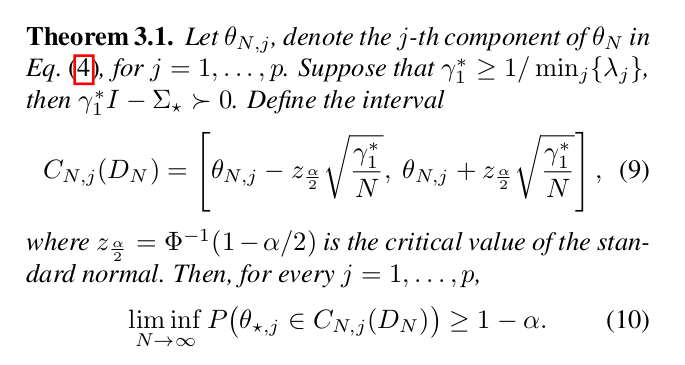
\includegraphics[scale=0.25]{31.png}
    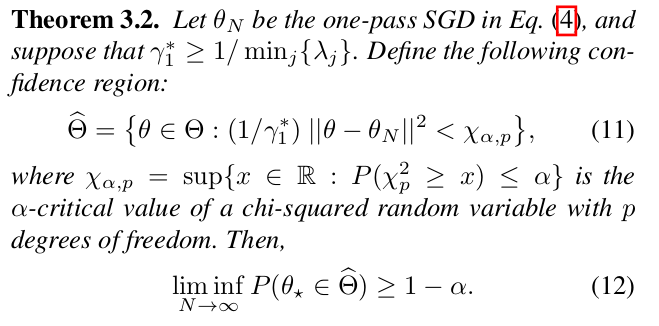
\includegraphics[scale=0.25]{32.png}
  \end{figure}
\end{frame}

\begin{frame}
  \frametitle{Summary of~\citet{chee:2023}}
  Selecting $\gamma_1^*$:
  \begin{figure}[h!]
    \centering
    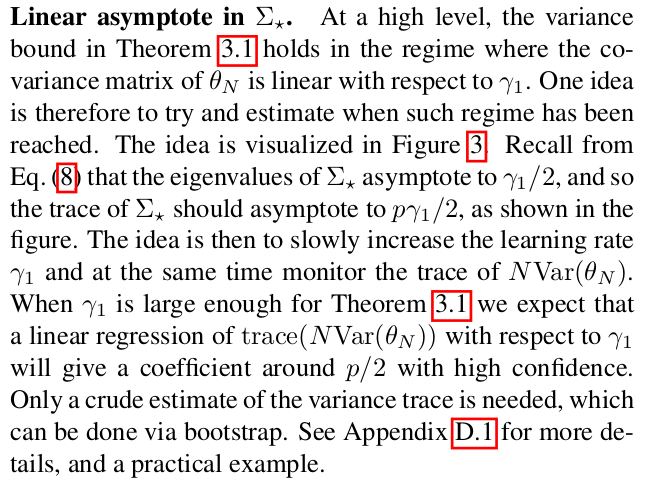
\includegraphics[scale=0.25]{s1.png}
    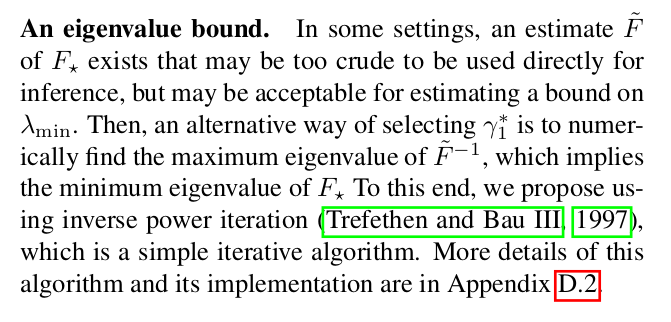
\includegraphics[scale=0.25]{s2.png}
  \end{figure}
\end{frame}


\begin{frame}
  \frametitle{Thresholding and SGD}
  \begin{itemize}
  \item In the context of thresholding we define the pivots
    \begin{align*}
      \frac{\hat{\beta}_j}{\sqrt{\frac{\gamma_1^*}{N}}}
    \end{align*}
    where we have the usual behaviour for $\hat{\beta}_j$ and the same behaviour from $\sqrt{\frac{\gamma_1^*}{N}} = O(N^{-1/2})$.
  \item Seems to work.
  \item Next steps: implementing an iterative version so we can build confidence sets. 
  \end{itemize}
\end{frame}

\begin{frame}
  \frametitle{Binomial, $p=10$, $s=5$}
  \begin{table}[h]
    \footnotesize
    \centering
    \begin{tabular}{l|r|r}
      Value & Proportion & Cumulative \\
      \hline
      (1,2,3,4,5) & 0.9132 & 0.9132 \\
      (1,3,4,5) & 0.0424 & 0.9556 \\
      () & 0.0162 & 0.9718 \\
      (1,4,5) & 0.0136 & 0.9854 \\
      (4,5) & 0.0050 & 0.9904 \\
      (1) & 0.0030 & 0.9934 \\
      (3) & 0.0030 & 0.9964 \\
      (1,3,5) & 0.0010 & 0.9974 \\
      (3,9) & 0.0010 & 0.9984 \\
      (1,3) & 0.0005 & 0.9989 \\
      (1,9) & 0.0005 & 0.9994 \\
      (9) & 0.0005 & 0.9999 \\
    \end{tabular}
    \caption{{\footnotesize $n=2000$, 95\% CS: \{(1,2,3,4,5), (1,3,4,5)\}}}
  \end{table}
\end{frame}

\begin{frame}
  \frametitle{Binomial, $p=100$, $s=5$}
  \begin{table}[h]
    \footnotesize
    \centering
    \begin{tabular}{l|r|r}
      Value & Proportion & Cumulative \\
      \hline
      (1,2,3,4,5) & 0.5786 & 0.5786 \\
      (1,2,3,4,5,29) & 0.1571 & 0.7357 \\
      () & 0.1016 & 0.8373 \\
      (1,2,3,4,5,28) & 0.0861 & 0.9234 \\
      (1,2,3,4,5,29,61) & 0.0311 & 0.9545 \\
      (1,3,4,5) & 0.0205 & 0.9750 \\
      (1,4) & 0.0061 & 0.9811 \\
      (1,2,3,4,5,61) & 0.0039 & 0.9850 \\
      (5) & 0.0039 & 0.9889 \\
      (1,2,3,4,5,7) & 0.0028 & 0.9917 \\
      (1) & 0.0028 & 0.9945 \\
      (4) & 0.0022 & 0.9967 \\
      (1,3,4) & 0.0017 & 0.9984 \\
      (1,3) & 0.0011 & 0.9995 \\
      (1,3,5) & 0.0006 & 1.0001 \\
    \end{tabular}
    \caption{{\footnotesize $n=2000$, 95\% CS: \{(1,2,3,4,5), (1,2,3,4,5,29), (), (1,2,3,4,5,28), (1,2,3,4,5,29,61)\}}}
  \end{table}
\end{frame}


\begin{frame}
  \frametitle{Binomial, $p=40$, $s=25$}
  \begin{table}[h]
    \tiny
    \centering
    \begin{tabular}{l|r|r}
      Value & Proportion & Cumulative \\
      \hline
       (1,2,3,4,5,6,7,8,9,10,11,12,13,14,15,16,17,18,19,20,21,22,23,24,25) & 0.2988 & 0.2988\\
                                                                  ()  & 0.1603& 0.4591\\
    (1,2,3,4,5,6,7,8,9,10,11,12,13,14,15,16,17,18,20,21,22,23,24,25)  &   0.1046 & 0.5637\\
                                                         (2,4,14,22)   &  0.0229 & 0.5866\\
                                                    (2,4,5,13,14,22)    & 0.0193 & 0.6059\\
                                                              (3,14)&     0.0187 & 0.6246\\
              (1,2,4,5,7,8,9,10,11,12,13,14,15,16,20,21,22,23,24,25) &    0.0167 & 0.6413\\
                                                            (3,4,14)  &   0.0146 & 0.6559\\
    (1,2,3,4,5,6,7,8,9,10,11,12,13,14,15,16,17,18,19,20,21,23,24,25)   &  0.0141 & 0.67\\
      (1,2,4,5,6,7,8,9,10,11,12,13,14,15,16,20,21,22,23,24,25)    & 0.0125 & 0.6825\\
      \vdots & \vdots & \vdots \\
    \end{tabular}
    \caption{{\tiny $n=2000$, 95\% CS: \{
        {(1,2,3,4,5,6,7,8,9,10,11,12,13,14,15,16,17,18,19,20,21,22,23,24,25), (), (1,2,3,4,5,6,7,8,9,10,11,12,13,14,15,16,17,18,20,21,22,23,24,25), (2,4,14,22), (2,4,5,13,14,22), (3,14), (1,2,4,5,7,8,9,10,11,12,13,14,15,16,20,21,22,23,24,25), (3,4,14), (1,2,3,4,5,6,7,8,9,10,11,12,13,14,15,16,17,18,19,20,21,23,24,25), (1,2,4,5,6,7,8,9,10,11,12,13,14,15,16,20,21,22,23,24,25), (1,2,4,6,7,8,9,10,11,12,13,14,15,16,17,19,20,21,22,23,24,25), (2,3,4,5,7,9,11,12,13,14,18,22,24,25), (1,2,3,4,5,6,7,8,10,11,12,13,14,15,17,18,20,21,22,23,24,25), (1,2,3,4,5,6,7,8,9,10,11,12,13,14,15,16,17,20,21,22,23,24,25), (1,2,3,4,5,7,8,9,10,11,12,13,14,15,16,17,18,20,21,22,23,24,25), (2,3,14), (3), (1,2,4,7,10,11,12,13,14,15,16,19,20,21,22,23,24,25), (2,14), (3,12,14), (2,4,14,19,22), (1,2,3,4,5,6,7,8,10,11,12,13,14,15,16,17,18,20,21,22,23,24,25), (1,2,3,4,5,6,7,8,9,10,11,12,13,14,15,16,17,18,19,20,21,22,24,25), (2,4,14,20,22), (3,9,12,14), (1,2,3,4,5,6,7,8,9,10,11,12,13,14,15,16,17,18,21,22,23,24,25), (1,2,4,5,7,10,11,12,13,14,15,16,19,20,21,22,23,24,25), (1,2,3,4,5,7,8,9,10,11,12,13,14,15,16,20,21,22,23,24,25), (1,2,4,7,10,11,12,13,14,15,16,19,20,21,22,24,25), (2,4,5,7,9,11,12,13,14,15,18,22,24,25), (1,2,4,5,7,10,11,12,14,15,16,19,20,21,22,23,24,25), (1,2,4,5,7,8,9,10,11,12,13,14,15,16,17,20,21,22,23,24,25), (1,2,4,5,7,9,10,11,12,13,14,15,16,18,19,20,21,22,23,24,25), (2,3,4,5,7,9,11,12,13,14,16,18,22,24,25), (1,2,3,4,7,8,9,10,11,12,13,14,15,16,17,18,20,21,22,24,25), (1,2,4,6,7,9,10,11,12,13,14,15,16,17,19,20,21,22,23,24,25), (1,2,5,7,9,10,11,12,13,14,15,16,18,19,20,21,22,23,24,25), (1,2,3,4,5,7,9,10,11,12,13,14,15,16,18,20,22,24,25), (1,2,4,5,13,14,22), (2,3,4,5,7,9,11,12,13,14,16,18,21,22,24,25), (1,2,3,4,5,6,7,8,10,11,12,13,14,15,16,17,20,21,22,23,24,25), (1,2,3,4,5,6,7,8,9,10,11,12,13,14,15,17,20,21,22,23,24,25), (1,2,3,4,5,7,8,9,10,11,12,13,14,15,16,17,18,20,21,22,24,25), (1,2,5,7,9,10,11,12,13,14,15,16,18,20,21,22,23,24,25), (2,3,4,5,7,9,10,11,12,13,14,15,16,18,21,22,24,25), (2,3,7,9,14,16,18,22,24,25), (1,2,4,7,8,9,10,11,12,13,14,15,16,17,19,20,21,22,23,24,25), (2,3,4,7,9,11,12,13,14,18,21,22,24,25), (2,3,5,7,8,9,14,15,16,18,21,22,24,25), (2,3,5,7,8,9,14,15,16,18,22,24,25), (1,2,3,4,5,6,7,8,9,10,11,12,13,14,15,16,17,18,20,21,22,24,25), (1,2,3,4,7,8,9,10,11,12,13,14,15,16,17,18,20,21,22,23,24,25), (1,2,4,5,7,9,10,11,12,13,14,15,16,18,19,20,22,23,24,25), (2,3,4,7,9,11,12,13,14,18,22,24,25), (1,2,3,7,8,9,14,15,16,18,22,24,25), (1,2,4,5,13,14,18,22,25), (1,2,4,5,7,10,11,12,13,14,15,16,19,20,21,22,24,25), (1,2,4,5,8,9,13,14,16,18,20,22,25), (1,2,4,7,8,10,11,12,13,14,15,16,19,20,21,22,24,25)}
        \}}}
  \end{table}
\end{frame}

\begin{frame}
  \frametitle{References}
  \bibliographystyle{chicago}
  \bibliography{sgd}
\end{frame}
\end{document}